\section{Light rays deviation}

\begin{figure}[H]
    \centering
    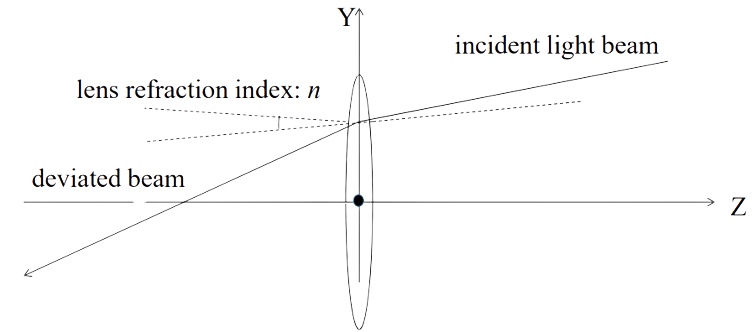
\includegraphics[width=0.4\linewidth]{images/ray.png}
\end{figure}
For a lens with a refractive index of $n$, the following equations hold true:
\[\dfrac{\theta-\alpha_1}{\theta^{'}-\alpha_1} \Rightarrow \dfrac{\sin{(\theta-\alpha_1)}}{\sin{(\theta^{'}-\alpha_1)}}=n\]
\[\dfrac{\theta^{''}-\alpha_2}{\theta^{'}-\alpha_2} \Rightarrow \dfrac{\sin{(\theta^{''}-\alpha_2)}}{\sin{(\theta^{'}-\alpha_2)}}=n\]
Where:
\begin{itemize}
    \item $\theta$ is the angle before the lens. 
    \item $\theta^{'}$ is the angle within the lens (not visible in the image). 
    \item $\theta^{''}$ is the angle after the lens.
\end{itemize}
By comparing these two equations, it is possible to determine the difference between the input angle $\theta$ and the output angle $\theta^{''}$, which can be expressed as:
\[\delta \theta=y(n-1)\left( \dfrac{1}{\rho_1} + \dfrac{1}{\rho_2}\right)\]
It is evident that the first term $(n-1)$is a result of the lens material, while the second term $\left( \frac{1}{\rho_1} + \frac{1}{\rho_2}\right)$ depends on the curvature of the lens surfaces.